\documentclass[12pt]{article}

%Russian-specific packages
%--------------------------------------
\usepackage[T2A]{fontenc}
\usepackage[utf8]{inputenc}
\usepackage[english, russian]{babel}
%for search in russian
\usepackage{cmap}
% for markdown style quotes
\usepackage{csquotes}
%--------------------------------------

%Math-specific packages
%--------------------------------------
\usepackage{amsmath}
\usepackage{amssymb}

\def\d{ \mathrm{d} }
\def\norm{ \mathrm{n} }

\usepackage{amsthm}
\newtheorem{lemma}{Лемма}
\newtheorem{definition}{Определение}
\newtheorem*{remark}{Замечание}

%Format-specific packages
%--------------------------------------
\usepackage[left=2cm,
            right=2cm,
            top=1cm,
            bottom=2cm,
            bindingoffset=0cm]{geometry}

%Graphics packages
%--------------------------------------
\usepackage{graphicx}
\usepackage{wrapfig}

\graphicspath{ { ./tex/ } }

\includeonly{
  tex/title
  , tex/introduction
}

\usepackage{tikz}
\usetikzlibrary{
  shapes.geometric
  , intersections
  , calc
  % for angles
  , angles
  , quotes
  , babel
  % ------
 , external
 , arrows.meta
 , patterns
}
\tikzexternalize[prefix=tex/]

\begin{document}

\begin{titlepage}
  \begin{center}
    \large{Федеральное государственное бюджетное образовательное\\
      учреждение высшего образования\\}

    Московский государственный университет\\
    имени М. В. Ломоносова\\

    \vspace{0.25 cm}

    \normalsize{Механико-математический факультет\\}
    \vspace{0.5 cm}
    Кафедра вычислительной математики\\
  \end{center}

  \vspace{3cm}

  \begin{center}
    \LARGE{Курсовая работа}\\

    \vspace{0.5 cm}

    \normalsize{}
    \textbf{Тема:} \textit{Введение в Photometric Stereo.}
  \end{center}

  \vspace{3 cm}

  \begin{flushright}
    \textbf{Выполнил:}\\
    студент 4 курса
    431 группы\\

    \textit{Шерстобитов Андрей Сергеевич}\\

    \vspace{1 cm}

    \textbf{Научный руководитель:}\\

    \textit{Валединский Владимир Дмитриевич}
  \end{flushright}

  \vspace{\fill}
  \normalsize{}
  \begin{center}
    Москва\\2022
  \end{center}

  \thispagestyle{empty}
\end{titlepage}


\newpage
\tableofcontents

\newpage

\section{Вступление}

Photometric stereo — метод в компьютерном зрении для определения
нормалей поверхности объектов путем наблюдения за этим объектом
при различных условиях освещения. Он основан на том факте,
что количество света, отражаемого поверхностью, зависит от ориентации
поверхности относительно источника света и наблюдателя.

\begin{figure}[h]
  \centering
  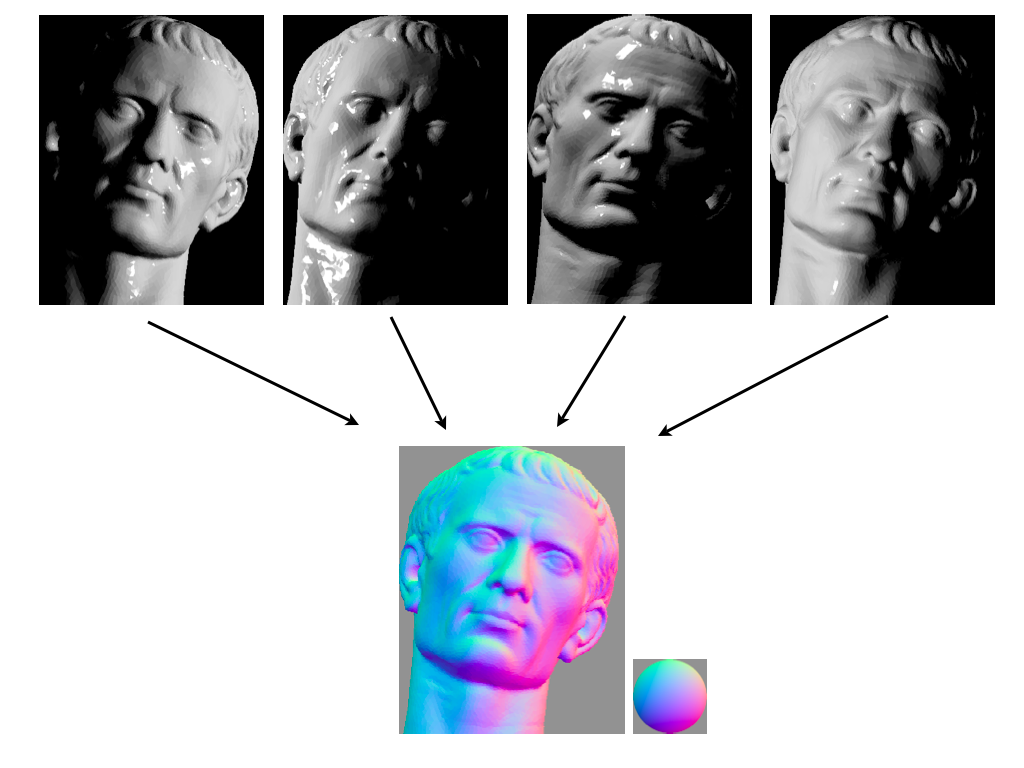
\includegraphics[scale=0.3]{tex/example.png}
\end{figure}

При использовании этого метода путем измерения количества света,
отраженного в камеру, пространство возможных ориентаций поверхности может
быть ограничено. Если объект наблюдается под достаточным количеством источников
света с разных углов, то ориентация поверхности может быть ограничена
до одной ориентации или даже получиться больше, чем необходимо.

Метод был впервые предложен в 1980 году Уодхэмом. Особый случай,
когда данные представлены одним изображением, известен как "shape from shading",
и был анализирован Б. К. П. Хорном в 1989 году. Расширенные методы фотометрического
стерео были разработаны для учета проецируемых теней и других
неоднородных условий освещения.

Однако, этот метод требует тщательного планирования и контроля эксперимента,
чтобы получить необходимое количество данных, и считается,
что он неэффективен для объектов с неоднородной поверхностью
и большим числом полостей. Тем не менее, photometric stereo все еще остается
важной технологией в области компьютерного зрения, особенно для задач
реконструкции трехмерных объектов.


\newpage

\section{Радиометрия}
\subsection{Телесный угол}

Познакомимся с понятием \textit{телесного угла}, разберемся как и в чем происходит измерение этой величины. Именно с него будет начинаться наше погружение
в Photometric stereo.

\begin{wrapfigure}[14]{r}{0.4\textwidth}
  \begin{center}
    \begin{tikzpicture}[scale=0.9,every node/.style={scale=0.9}]
      \draw (0,0) circle (2cm);
      \coordinate [label=below:$O$] (O) at (0,0);
      \draw [dashed] (0,0) -- node[above]{$R$} (-2,0);
      \draw (-2,0) arc (180:360:2 and 0.6);
      \draw [dashed] (2,0) arc (0:180:2 and 0.6);

      \node [ellipse,
        draw=black,
        fill=cyan!10,
        minimum width = 0.6cm,
        minimum height = 0.4cm,
        rotate=125] (e) at (0.9,0.9) {};
      \draw [dashed] (O) -- (e.east);
      \draw [dashed] (O) -- (e.west);

      \node [ellipse,
        draw=black,
        fill=cyan!20,
        minimum width = 1.8cm,
        minimum height = 1.2cm,
        rotate=125] (E) at (2.70,2.70) {};
      \draw (e.east) -- (E.east);
      \draw (e.west) -- (E.west);
      \coordinate [label=center:$\Sigma$] (S) at (E.center);

    \end{tikzpicture}
    \caption{Телесный угол}
  \end{center}
\end{wrapfigure}

Поставим наблюдателя в центр сферы $O$ радиуса $R$. Обозначим $\Sigma$ наблюдаемую
из точки $O$ поверхность. Площадь сферы покрываемую объектом обозначим $S$. Тогда величиной телесного угла
является следующее отношение:
$$\omega=\frac{S}{R^2}$$
Точка $O$ называется вершиной (apex) телесного угла.
\textbf{Телесный угол} - пучок лучей из $O$ до $\Sigma$.
Говорят, что наблюдатель \textit{стягивает} его телесный угол в вершине.

Единица измерения в системе  СИ - стерадиан (ср, sr), равный телесному углу,
вырезающему из сферы радиуса $R$ поверхность с площадью $R^2$.

\begin{remark}
  Площадь поверхности сферы = $4\pi R^2$, тогда полный телесный угол равен
  $$\omega=\frac{4\pi R^2}{R^2}=4\pi$$
\end{remark}

\begin{remark}
  Для кругового конуса с углом раствора $\theta$ телесный угол при его вершине
  равен $$\omega=\frac{2\pi R^2(1-\cos\theta)}{R^2}=2\pi(1-\cos\theta)$$
\end{remark}

\begin{wrapfigure}[10]{r}{0.35\textwidth}
  \begin{center}
    \begin{tikzpicture}[scale=0.75]
      \coordinate (O) at (0,0);
      \node [circle,
        name path=U,
        draw=black,
        minimum size=3cm] (U) at (O) {};
      \node [circle,
        draw=black,
        label=left:$S_0$] (S0) at (O) {};

      \coordinate (dAl) at (1,-7);
      \coordinate (dAr) at (3,-7);
      \coordinate (dAm) at ($(dAl)!0.5!(dAr)$);
      \coordinate (n) at (2,-6);
      \draw (dAl) -- (dAr);

      \draw [name path=O--dAl,dashed] (O) -- node [left] {$r$} (dAl);
      \draw [name path=O--dAr,dashed] (O) -- (dAr);
      \draw (O) -- (dAm) node [below] {$\d A$};

      \begin{scope}
        \path [name intersections={of=O--dAl and U,by=C}];
        \path [name intersections={of=O--dAr and U,by=D}];
        \draw [line width=1mm] (C) -- (D) node [right] {$\d A_0$};
      \end{scope}

      \draw [->, line width=0.5mm] (dAm) -- (n) node [right] {$\norm$};
      \pic [draw, angle radius=6mm,"$\theta$",left] {angle=n--dAm--O};
    \end{tikzpicture}
    \caption{Стянутый объектом $S_0$ телесный угол}
    \label{subtended}
  \end{center}
\end{wrapfigure}

Чаще всего бывает, что изучаемая поверхность находится под углом $\theta$
к наблюдателю. На рис. \eqref{subtended} $\norm$ это нормаль к
изучаемой поверхности $\d A$, $S_0$ - центр единичной окружности.
Расстояние между $S_0$ и $\d A$ обозначим $r$. Заметим, что угол между
нормалью плоскости $\norm$ и направлением взгляда наблюдателя обозначим $\theta$.
$\d A_0$ является проекцией $\d A$ на единичную сферу, тогда телесный угол имеет величину:
$$\d \omega = \frac{\d A\cos\theta}{r^2}$$

\newpage

\subsection{Сила света (Intensity)}

Простыми словами фотометрия - наука об измерении света с точки
зрения его яркости, воспринимаемой человеческим глазом.
Сразу можно задать вопрос: как и в чем измеряется
свет? Попытаемся формализировать ответы на эти вопросы.

Современное определение единицы силы света было зафиксировано в 1979 г.
XVI Генеральной конференцией по мерам и весам. Международной системе единиц (СИ)
имеет следующее описание:

\begin{displayquote}
  Сила света в заданном направлении источника, испускающего
  монохроматическое излучение частотой 540$\cdot$1012 Гц, энергетическая сила света
  которого в этом направлении составляет 1/683 Вт/ср.
\end{displayquote}

Единица силы света имеет общеприниятое название -- кандела (кд, cd).
Сила света имеет обозначение $I$.

Для силы света оказался верен закон обратных квадратов: значение силы света в
данной точке пространства обратно пропорицонально квадрату расстояния от источника света.
То есть имея два источника света с соотвествующими силами $I_1$ и $I_2$, расположенные
соответственно на расстояних $r_1$ и $r_2$ верно следующее равенство:

\begin{equation} \label{inverse_law}
  \frac{I_1}{I_2} = \frac{r_2^2}{r_1^2}
\end{equation}

\subsection{Поток (Flux)}

Рассмотрим некоторый источник света $S_0$ в некотором пространстве.
Излучаемый свет можно представить как совокупность телесных углов $\omega$ с вершиной
в источнике $S_0$. Пусть источник света имеет силу $I$.

\begin{figure}[h]
  \begin{center}
    \begin{tikzpicture}[
        declare function={lin(\t) = \t / 1.5;}
      ]
      \newcommand\connectEllipces[3]{
        \path [name intersections={of=S0--omega_east and #1,by=A}];
        \path [name intersections={of=S0--omega_west and #1,by=B}];
        \draw
        (#2) -- (A)
        (#3) -- (B);
      };

      \def \R {115};
      \tikzstyle{ellipse template}=[ellipse,draw=black,minimum width=1cm,minimum height=0.5cm,rotate=\R];

      \coordinate [label=left:$S_0$] (S0) at (0, 0);

      \def \OmegaScale {1};
      \path let \n1={8} in node [ellipse template
          , fill=gray
          , opacity=0.3
          , scale=\OmegaScale
          , name path=omega
        ] (omega) at (\n1,{ lin(\n1) }){};
      \node at (omega.center) {$\omega$};
      \coordinate (S0_omega_west_vector) at ($ (omega.west) - (S0) $);

      \draw [name path=S0--omega_east,dashed] (S0) -- (omega.east);
      \draw [name path=S0--omega_west,dashed] (S0) -- (omega.west);

      \path let \n1={2.4} in node [ellipse template
          , scale=1.5
          , name path=e] (e) at (\n1,{ lin(\n1) }) {};

      \draw [->] (S0) -- node [left] {$r_1$} (e.north east);
      \connectEllipces{e}{S0}{S0};

      \path [name path=e_vert] (e.west) -- (e.east);
      \path [name intersections={of=S0--omega_east and e_vert,by=e_omega_east}];
      \path [name intersections={of=S0--omega_west and e_vert,by=e_omega_west}];
      \path let
      \n1 = {2.4},
      \p2 = (S0_omega_west_vector),
      \p3 = ($ (e_omega_west) - (S0) $),
      \n4 = { veclen(\x3,\y3) / veclen(\x2,\y2) }
      in node [ellipse template
          , scale=\OmegaScale * \n4
          , name path=e_omega
        ] (e_omega) at (\n1,{ lin(\n1) }) {};
      \node [below] at (e_omega_west) {$\sigma_1$};

      \path let \n1={3.6} in node [ellipse template
          , scale=2.5
          , name path=E] (E) at (\n1,{ lin(\n1) }) {};

      \draw [->] (S0) -- node [below] {$r_2$} (E.north west);
      \connectEllipces{E}{e_omega_east}{e_omega_west};

      \path [name path=E_vert] (E.west) -- (E.east);
      \path [name intersections={of=S0--omega_east and E_vert,by=E_omega_east}];
      \path [name intersections={of=S0--omega_west and E_vert,by=E_omega_west}];
      \path let
      \n1 = {3.6},
      \p2 = (S0_omega_west_vector),
      \p3 = ($ (E_omega_west) - (S0) $),
      \n4 = { veclen(\x3,\y3) / veclen(\x2,\y2) }
      in node [ellipse template
          , scale=\OmegaScale * \n4
          , name path=E_omega
        ] (E_omega) at (\n1,{ lin(\n1) }) {};
      \node [below] at (E_omega_west) {$\sigma_2$};

      \path let \n1={5.6} in node [ellipse template
          , scale=4
          , name path=EE] (EE) at (\n1,{ lin(\n1) }) {};

      \draw [->] (S0) -- node [below] {$r_3$} (EE.west);
      \connectEllipces{EE}{E_omega_east}{E_omega_west};

      \path [name path=EE_vert] (EE.west) -- (EE.east);
      \path [name intersections={of=S0--omega_east and EE_vert,by=EE_omega_east}];
      \path [name intersections={of=S0--omega_west and EE_vert,by=EE_omega_west}];
      \path let
      \n1 = {5.6},
      \p2 = (S0_omega_west_vector),
      \p3 = ($ (EE_omega_west) - (S0) $),
      \n4 = { veclen(\x3,\y3) / veclen(\x2,\y2) }
      in node [ellipse template
          , scale=\OmegaScale * \n4
          , name path=EE_omega
        ] (EE_omega) at (\n1,{ lin(\n1) }) {};
      \node [below] at (EE_omega_west) {$\sigma_3$};

      \draw
      (EE_omega_east) -- (omega.east)
      (EE_omega_west) -- (omega.west);

    \end{tikzpicture}
    \caption{Световой поток источника $S_0$ внутри угла $\omega$}
  \end{center}
\end{figure}

Произвольными радиусами $r_1$, $r_2$, $r_3$ построим сферы с центром в вершине
телесного угла $S_0$ и обозначим выделенные телесным углом площади на сферах соответсвенно
$\sigma_1$, $\sigma_2$, $\sigma_3$. За единицу времени на эти площади упадет одна и та
же энергия: $\frac{I}{r_1^2}\sigma_1$, $\frac{I}{r_2^2}\sigma_2$, $\frac{I}{r_3^2}\sigma_3$.
Обратим внимание, что $\frac{\sigma_1}{r_1^2}=\frac{\sigma_2}{r_2^2}=\frac{\sigma_3}{r_3^2}=\omega$.
Таким образом, \textbf{поток} - физическая величина пропорциональная световой мощности,
переносимой пучком лучей, распространяющимися внутри телесного угла $\omega$.
\[\Phi:=I\omega\]
Световой поток, выходящий из телесного угла 1ср, с силой света 1кд называется \textit{люмен} (лм, lm).

Обратим внимание, что в качестве источника света здесь рассматривается вершина телесного угла, то есть
точка в пространстве, но в жизни же источники света не только не могут быть точкой, но и могут
достигать весьма больших размеров. Всегда стоит помнить, что если речь идет об источнике света
как о точке, то подразумевается, что расстояние между освещаемым объектом во много раз
превышает размер источника и, в следствие различные лучи источника попадают в достаточно малый телесный угол.

\subsection{Освещенность (Irradiance)}

Зафиксируем точечный источник света $S_0$ с силой света $I$ на расстоянии $r$ от поверхности площадью $\sigma$.
\begin{figure}[h]
  \begin{center}
    \begin{tikzpicture}
      \node [circle,
        draw=black,
        scale=0.4,
        label=left:$S_0$] (S0) at (0,0) {};
      \coordinate (S0) at (S0);

      \coordinate (Au) at (7,1);
      \coordinate (Al) at (7,-1);
      \draw (Au) -- node[right]{$\sigma$} (Al);
      \draw (Au) -- (S0) -- (Al);
      \draw [-{Stealth[scale=2]}] (S0) -- node[above]{$r$} ($(Au)!0.5!(Al)$);
    \end{tikzpicture}
    \caption{Лучи $S_0$, падающие по нормали к поверхности}
  \end{center}
\end{figure}

Величина
\begin{equation}\label{irradiance}
  E:=\frac{I}{r^2}
\end{equation}

является мерой освещения, получающегося на поверхности при падении лучей под прямым углом.

За единицу освещенности принимается такая освещенность, которую создает
источник силой света в 1 кд, освещающий по нормали поверхность,
отстояющую от него на расстояние 1 м. Единица освещенности — люкс (лк, lx).

Проводя аналогии с физическими величинами, можно сравнить освещенность с плотностью потока.
Действительно, домножив числитель и знаменатель \eqref{irradiance} на бесконечно малый телесный
угол $\d\omega$, получим следующее

\[E=\frac{I\d\omega}{r^2\d\omega}=\frac{\d\Phi}{\d\sigma}\]

\begin{figure}[h]
  \begin{center}
    \begin{tikzpicture}
      \node [circle,
        draw=black,
        scale=0.4,
        label=left:$S_0$] (S0) at (0,0) {};
      \coordinate (S0) at (S0);

      \coordinate (Au) at (7,1);
      \coordinate (Al) at (9,-1);
      \coordinate (Am) at ($(Au)!0.5!(Al)$);
      \path let \p1=($ (Au) - (Al) $) in node (N) at ([shift={(-\y1,\x1)}]Am){$N$};
      \draw (Au) -- node[right,scale=1.5]{$\frac{\sigma}{\cos\phi}$} (Al);
      \draw (Au) -- (S0) -- (Al);
      \draw [-{Stealth[scale=2]}] (S0) -- node[above]{$r$} (Am);
      \draw [-{Stealth[scale=2]}] (Am) -- (N);
      \pic [draw, angle radius=20mm,"$\phi$",left] {angle=S0--Am--N};
    \end{tikzpicture}
    \caption{Лучи $S_0$, падающие под углом $\phi$}
    \label{irradiance_under_angle}
  \end{center}
\end{figure}

В случае, когда лучи источника падают под углом $\phi$ к нормали на Рис. \eqref{irradiance_under_angle}, сила светового
потока распределяется по увеличнной площади, в следствие чего освещенность поверхности
оказывается меньше:

\begin{equation}
  E=\frac{\d\Phi}{\d\sigma/\cos\phi}=\frac{I}{r^2}\cos\phi
\end{equation}

\subsection{Энергетическая яркость (Radiance)}

На рисунке \eqref{radiance_pic} в качестве источника рассматривается бесконечно
малая площадь поверхности $\d\sigma_1$, в качестве получателя рассматривается бесконечно
малая площадь поверхности $\d\sigma_2$, расстояние между ними конечно и равно $r$.
Пусть нормаль $\norm_1$ поверхности $\d\sigma_1$ образует с пучком света угол $\phi_1$,
нормаль $\norm_2$ соответсвенно $\phi_2$.

\begin{figure}[h]
  \begin{center}
    \begin{tikzpicture}
      \tikzstyle{trapezium template}=[trapezium, draw, minimum width=3cm, trapezium left angle=120, trapezium right angle=60, scale=0.5]

      \node [trapezium template, rotate=30] (L) at (0, 0){};
      \node [trapezium template, rotate=-30] (R) at (7, 0){};
      \node [draw=black,circle,scale=0.3] (Lc) at (L.center){};
      \node [draw=black,circle,scale=0.3] (Rc) at (R.center){};

      \draw [-{Stealth[scale=2]}] (Lc) -- node[above]{$r$} (Rc);

      \path let \p1=($ (L.north) - (L.south) $) in node (LN) at ([shift={(1.5,1.5)}]Lc){$\norm_1$};
      \draw [->] (Lc) -- (LN);
      \pic [draw, angle radius=12mm,"$\phi_1$"] {angle=Rc--Lc--LN};

      \path let \p1=($ (R.north) - (R.south) $) in node (RN) at ([shift={(-1.5,-1.5)}]Rc){$\norm_2$};
      \draw [->] (Rc) -- (RN);
      \pic [draw, angle radius=12mm,"$\phi_2$"] {angle=Lc--Rc--RN};

    \end{tikzpicture}
    \caption{Световой поток пластинки $\d\sigma_1$ на $\d\sigma_2$}
    \label{radiance_pic}
  \end{center}
\end{figure}

По определению световой поток должен быть пропорционален площадям
проекций каждой из площадок $\d\sigma_1$ и $\d\sigma_2$ на плоскость,
перпендикулярную направлению падающего пучка, и обратно пропорционален квадрату
расстояния между ними. Его можно представить в следующей форме

\begin{equation}\label{radiance::origin}
  \d^2\Phi=L\frac{\d\sigma_1\cos\phi_1\d\sigma_2\cos\phi_2}{r^2}
\end{equation}

Коэффициент пропорциональности $L$
называется \textbf{яркостью} излучающего элемента $\d\sigma_1$ в направлении
к освещаемому элементу $\d\sigma_2$.

Рассмотрим выражение \eqref{radiance::origin} иначе. Возьмем за источник $\d\sigma_1$ с силой $\d I$,
тогда световой поток, падающий на пластинку $\d\sigma_2$, можно представить следующим образом:
\begin{equation}\label{radiance::flux_on_receiver}
  \d^2\Phi=\d E_2\d\sigma_2=\frac{\d I}{r^2}\cos\phi_2\d\sigma_2
\end{equation}
Из \eqref{radiance::origin} и \eqref{radiance::flux_on_receiver} следует
\begin{equation}\label{radiance::result}
  L = \frac{\d I}{\d\sigma_1\cos\phi_1}
\end{equation}

Выражение \eqref{radiance::result} определяет \textit{яркость поверхности в заданной точке
  и в заданном направлении}. Единица яркости -- кандела на квадратный метр (кд/м$^2$).


\newpage

\section{Поверхности}

\subsection{Двулучевая функция отражательной способности (BRDF)}

Очевидно, что яркость точки на поверхности как-то зависит от материала поверхности,
на которую падает свет. Иначе говоря, яркость зависит от так называемых отражательных
способностей поверхности. На Рис. \eqref{brdf} компьютером отрисованы различные сферы.
В данном примере и камера и источник света находятся относительно далеко от сфер.
Причина, по которой мы видим их различными -- их материал, или различные отражательные способности.

\begin{figure}[h]
  \centering
  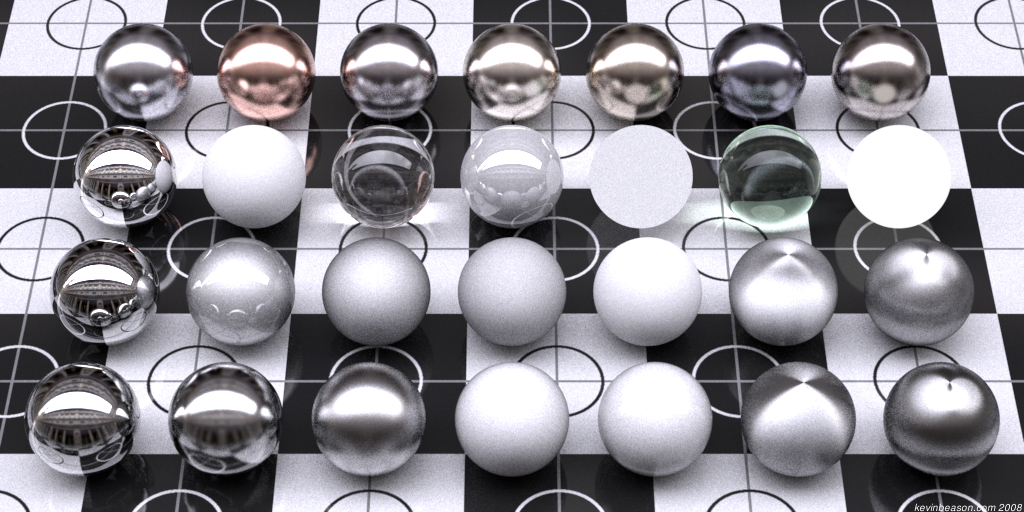
\includegraphics[scale=0.3]{tex/brdf.png}
  \caption{Пример разных отражательных способностей}
  \label{brdf}
\end{figure}

Возникает идея как-то формализировать представление отражательных способностей любого материала,
с чем нам поможет двулучевая функция отражательной способности или ДФОС.

Для определения нам важны направления: направление света, падающего на предмет, и направление
отраженного и полученного света. Двулучевая функция, потому что речь будет идти про два луча.

\begin{figure}[h]
  \begin{center}
    \begin{tikzpicture}
      \def\SndrAngle {225};
      \def\SndrColor {yellow};
      \node [draw,
        fill=\SndrColor,
        rectangle,
        minimum width=1cm,
        minimum height=0.5cm,
        rotate=\SndrAngle,
      ] (SndrRect) at (-5, 4){};
      \filldraw[fill=\SndrColor] let
      \p1=($ (SndrRect.north west) - (SndrRect.north east) $),
      \n2={0.3}
      in
      ($ (SndrRect.north east)!.5!(SndrRect.north) $) coordinate (SndrA) --
      ($ (SndrRect.north)!.5!(SndrRect.north west) $) coordinate (SndrB) --
      ([shift={(\y1*\n2,-\x1*\n2)}]SndrRect.north west) coordinate (SndrC) --
      ([shift={(\y1*\n2,-\x1*\n2)}]SndrRect.north east) coordinate (SndrD) -- cycle
      ;
      \node[left,text width=2.5cm] at (SndrRect.south east) {Источник (Прожектор)};

      \def\RcvrColor {gray};
      \node [draw,
        fill=\RcvrColor,
        rectangle,
        minimum width=1cm,
        minimum height=0.5cm,
        rotate=360-\SndrAngle,
      ] (RcvrRect) at (5, 4){};
      \filldraw[fill=\RcvrColor] let
      \p1=($ (RcvrRect.north west) - (RcvrRect.north east) $),
      \n2={0.3}
      in
      ($ (RcvrRect.north east)!.5!(RcvrRect.north) $) coordinate (RcvrA)
      -- ($ (RcvrRect.north)!.5!(RcvrRect.north west) $) coordinate (RcvrB)
      -- ([shift={(\y1*\n2,-\x1*\n2)}]RcvrRect.north west) coordinate (RcvrC)
      -- ([shift={(\y1*\n2,-\x1*\n2)}]RcvrRect.north east) coordinate (RcvrD)
      -- cycle
      ;
      \node[right,text width=2.5cm] at (RcvrRect.south west) {Получатель (Камера)};

      \node [draw,
        trapezium,
        shade,
        minimum width=3cm,
        trapezium left angle=120,
        trapezium right angle=60] (Srfc) at (0, 0){};

      \draw[-Stealth, thick]
      (Srfc.center) coordinate (beginN)
      -- ([shift={(0,1.5)}]Srfc.center) coordinate (endN) node[above]{$\norm$};

      \draw[-Stealth,color=\SndrColor,line width=0.5mm]
      ($ (SndrC)!.5!(SndrD) $) coordinate (beginSnd)
      --node[left,color=black]{$(\theta_i,\phi_i)$} (Srfc.center) coordinate (endSnd);

      \draw[-Stealth,color=\RcvrColor,line width=0.5mm]
      (Srfc.center) coordinate (beginRcv)
      --node[right,color=black]{$(\theta_r,\phi_r)$} ($ (RcvrC)!.5!(RcvrD) $) coordinate (endRcv);

    \end{tikzpicture}
    \caption{Отражение поверхности}
    \label{surface_reflection}
  \end{center}
\end{figure}

Таким образом, чтобы представить свойства отражения любого материала,
мы хотим иметь возможность описать его свойства как с точки зрения
направления освещения, так и с точки зрения направления взгляда или направления отражения.

Выражая направление источника в полярных координатах через углы $(\theta_i,\phi_i)$ и
направление отраженного света через $(\theta_r,\phi_r)$, мы можем следующее
\begin{enumerate}
  \item Освещенность поверхности зависит от углов $(\theta_i,\phi_i)$, то есть $E:=E(\theta_i,\phi_i)$.
  \item Яркость поверхности зависит от углов $(\theta_r,\phi_r)$, то есть $L:=L(\theta_r,\phi_r)$.
\end{enumerate}

И теперь мы можем описать отражательную способность как двулучевую функцию отражательной
способноси:
\begin{equation}
  \rho(\theta_i,\phi_i,\theta_r,\phi_r)=\frac{L(\theta_r,\phi_r)}{E(\theta_i,\phi_i)}
\end{equation}

Измеряется в ср$^{-1}$, где стерадиан (ср) - единица измерения телесного угла. Перечислим некоторые свойства ДФОС:
\begin{enumerate}
  \item Неотрицательность: $\rho(\theta_i,\phi_i,\theta_r,\phi_r)>0$. Следует из того, что и
        яркость, и освещенность неотрицательны, значит и их отношение.
  \item Удовлетворяет равенству Гельмгольца: $\rho(\theta_i,\phi_i,\theta_r,\phi_r)=\rho(\theta_r,\phi_r,\theta_i,\phi_i)$.
        Это нам говорит о том, что поменяв местами прожектор и камеру, мы получим то же самое значение ДФОС.
\end{enumerate}

Существуют множество поверхностей, которые отражают одинаковое количество света
вне зависимости от вращения этой поверхности вокруг ее нормали. Такие
поверхности называют \textit{изотропными}, в обратном случае \textit{анизотропными}.
Когда говорят об изотропных поверхностях ДФОС определяют как функцию принимающую три
аргумента вместо четырех: $\rho(\theta_i,\theta_r,\phi)$.

\subsection{Механизмы, порождающие отражение}

Давайте поговорим об основных механизмах, порождающие отражение света.

\begin{figure}[h]
  \centering
  \begin{minipage}{.5\textwidth}
    \centering
    \begin{tikzpicture}
      \node [draw,
        rectangle,
        minimum width=6cm,
        minimum height=0.5cm,
      ] (obj) at (0, -1){};

      \draw[-Stealth, thick, black] (-3,3) coordinate (src) --node[above, midway, sloped]{Источник} ($ (obj.north east)!.5!(obj.north west) $) coordinate (middle);
      \draw[-Stealth, thick, blue] (middle) --node[above, midway, sloped]{Зеркальное отражение} (3,3) coordinate;
    \end{tikzpicture}
  \end{minipage}%
  \begin{minipage}{.5\textwidth}
    \centering
    \begin{tikzpicture}
      \node [draw,
        rectangle,
        pattern=bricks,
        minimum width=6cm,
        minimum height=1cm,
      ] (obj) at (0, -1){};
      \draw[-Stealth, thick, black] (-3,3) coordinate (src) --node[above, midway, sloped]{Источник} ($ (obj.north east)!.5!(obj.north west) $) coordinate (middle);
      \node [circle,
        inner sep=0pt,
        outer sep=0pt,
        minimum size=3cm] (C1) at (0,1) {};
      \draw[-Stealth, thick, red] (middle) -- (C1.north) coordinate node[right]{Диффузное отражение};
      \draw[-Stealth, thick, red] (middle) -- (C1.north west) coordinate;
      \draw[-Stealth, thick, red] (middle) -- (C1.north east) coordinate;
      \draw[-Stealth, thick, red] (middle) -- (C1.west) coordinate;
      \draw[-Stealth, thick, red] (middle) -- (C1.east) coordinate;
      \draw[-Stealth, thick, red] (middle) -- (C1.south west) coordinate;
      \draw[-Stealth, thick, red] (middle) -- (C1.south east) coordinate;
      \node [circle,
        inner sep=0pt,
        outer sep=0pt,
        rotate=22.5,
        minimum size=3cm] (C2) at (0,1) {};
      \draw[-Stealth, thick, red] (middle) -- (C2.north) coordinate;
      \draw[-Stealth, thick, red] (middle) -- (C2.north west) coordinate;
      \draw[-Stealth, thick, red] (middle) -- (C2.north east) coordinate;
      \draw[-Stealth, thick, red] (middle) -- (C2.west) coordinate;
      \draw[-Stealth, thick, red] (middle) -- (C2.east) coordinate;
      \draw[-Stealth, thick, red] (middle) -- (C2.south) coordinate;
      \draw[-Stealth, thick, red] (middle) -- (C2.south west) coordinate;
      \draw[-Stealth, thick, red] (middle) -- (C2.south east) coordinate;
    \end{tikzpicture}
  \end{minipage}
  \caption{Диффузное и зеркальное отражение}
  \label{reflect}
\end{figure}

Рассмотрим рис. \eqref{reflect}. Различают три механизма:
\begin{itemize}
  \item Первый - отражательная способность поверхности. Свет падает на поверхность
        и отражение происходит на самой плоскости. Такое отражение света называется
        \textit{зеркальны м} отражением. Оно придает поверхностям глянцевый или блестящий
        вид и свойственно гладким однородным материалам (зеркалам, стеклу, полированным металлам).
  \item Второй случай возникает, когда часть света проходит сквозь поверхность
        и проникает внутрь материала. Обычно вещества неоднородны и содержат различные
        частицы с разными показателями преломления. В результате попадающий внутрь свет
        преломляется и отражается несколько раз, отскакивает внутри случайным образом.
        Это происходит на небольшой глубине под поверхностью, поэтому частицы света
        проникают обратно и рассеиваются во многих направлениях.
        Это явление называется \textit{диффузным}. Из-за неоднородности среды
        объекты обладают матовостью.
  \item При анализе яркости точки изображения надо учитывать, что это результат отражения света из окружающей среды, который имеет составляющие
        диффузного и поверхностного отражения. Чаще всего встречается \textit{гибридное} отражение — комбинация этих двух механизмов.
\end{itemize}
\subsection{Закон Ламберта}

\section{Photometric stereo}

\subsection{Постановка задачи}
\subsection{Решение для поверхностей Ламберта}
\subsection{Проблемы, возможные решения}

\section{Литература}
\begin{enumerate}
  \item Гуревич М. М. Фотометрия. Теория, методы и приборы. — 2-е изд. — Л.: Энергоатомиздат. Ленинградское отделение, 1983. — С. 23—24. — 272 с.
  \item Ying Wu. "Radiometry, BRDF and Photometric Stereo". Northwestern University. Retrieved 2015-03-25.
  \item A. V. Arecchi, T. Messadi, and R. J. Koshel, Field Guide to Illumination, SPIE Press, Bellingham, WA (2007)
\end{enumerate}
\end{document}
